\section{Results}
\label{sec:results}

\subsection{Marginal adequacy}

The marginal stage produces a clear split between the commodity series and the cedi. Under both calendar constructions, each of the four commodities has at least one candidate that passes the stated residual, squared-residual and PIT adequacy gates. The cedi does not. In both panels the selected cedi specification is therefore an inadequate reference model rather than an adequate marginal representation. This distinction is carried into every cedi-related copula and EVT interpretation.

The calendar choice nevertheless changes the return process itself. Panel A contains materially more exact zero returns because carried prices create zero movements on some business days; the cedi zero share is 22.27\% in Panel A and 16.51\% in Panel B. The persistence of a high zero share in Panel B indicates that the cedi marginal problem cannot be attributed solely to forward filling.

\subsection{Finite-threshold tail concentration}

Figure~\ref{fig:tail-profiles} reports the empirical lower- and upper-tail concentration measures at \(q=0.025\), \(0.05\) and \(0.10\) for representative pairs in both panels. The profiles are treated as finite-threshold summaries, not as estimates of asymptotic tail-dependence coefficients. Their role is descriptive: the formal stress inference is based on the moving-block-bootstrap differences reported below.

\begin{figure}[htbp]
\centering
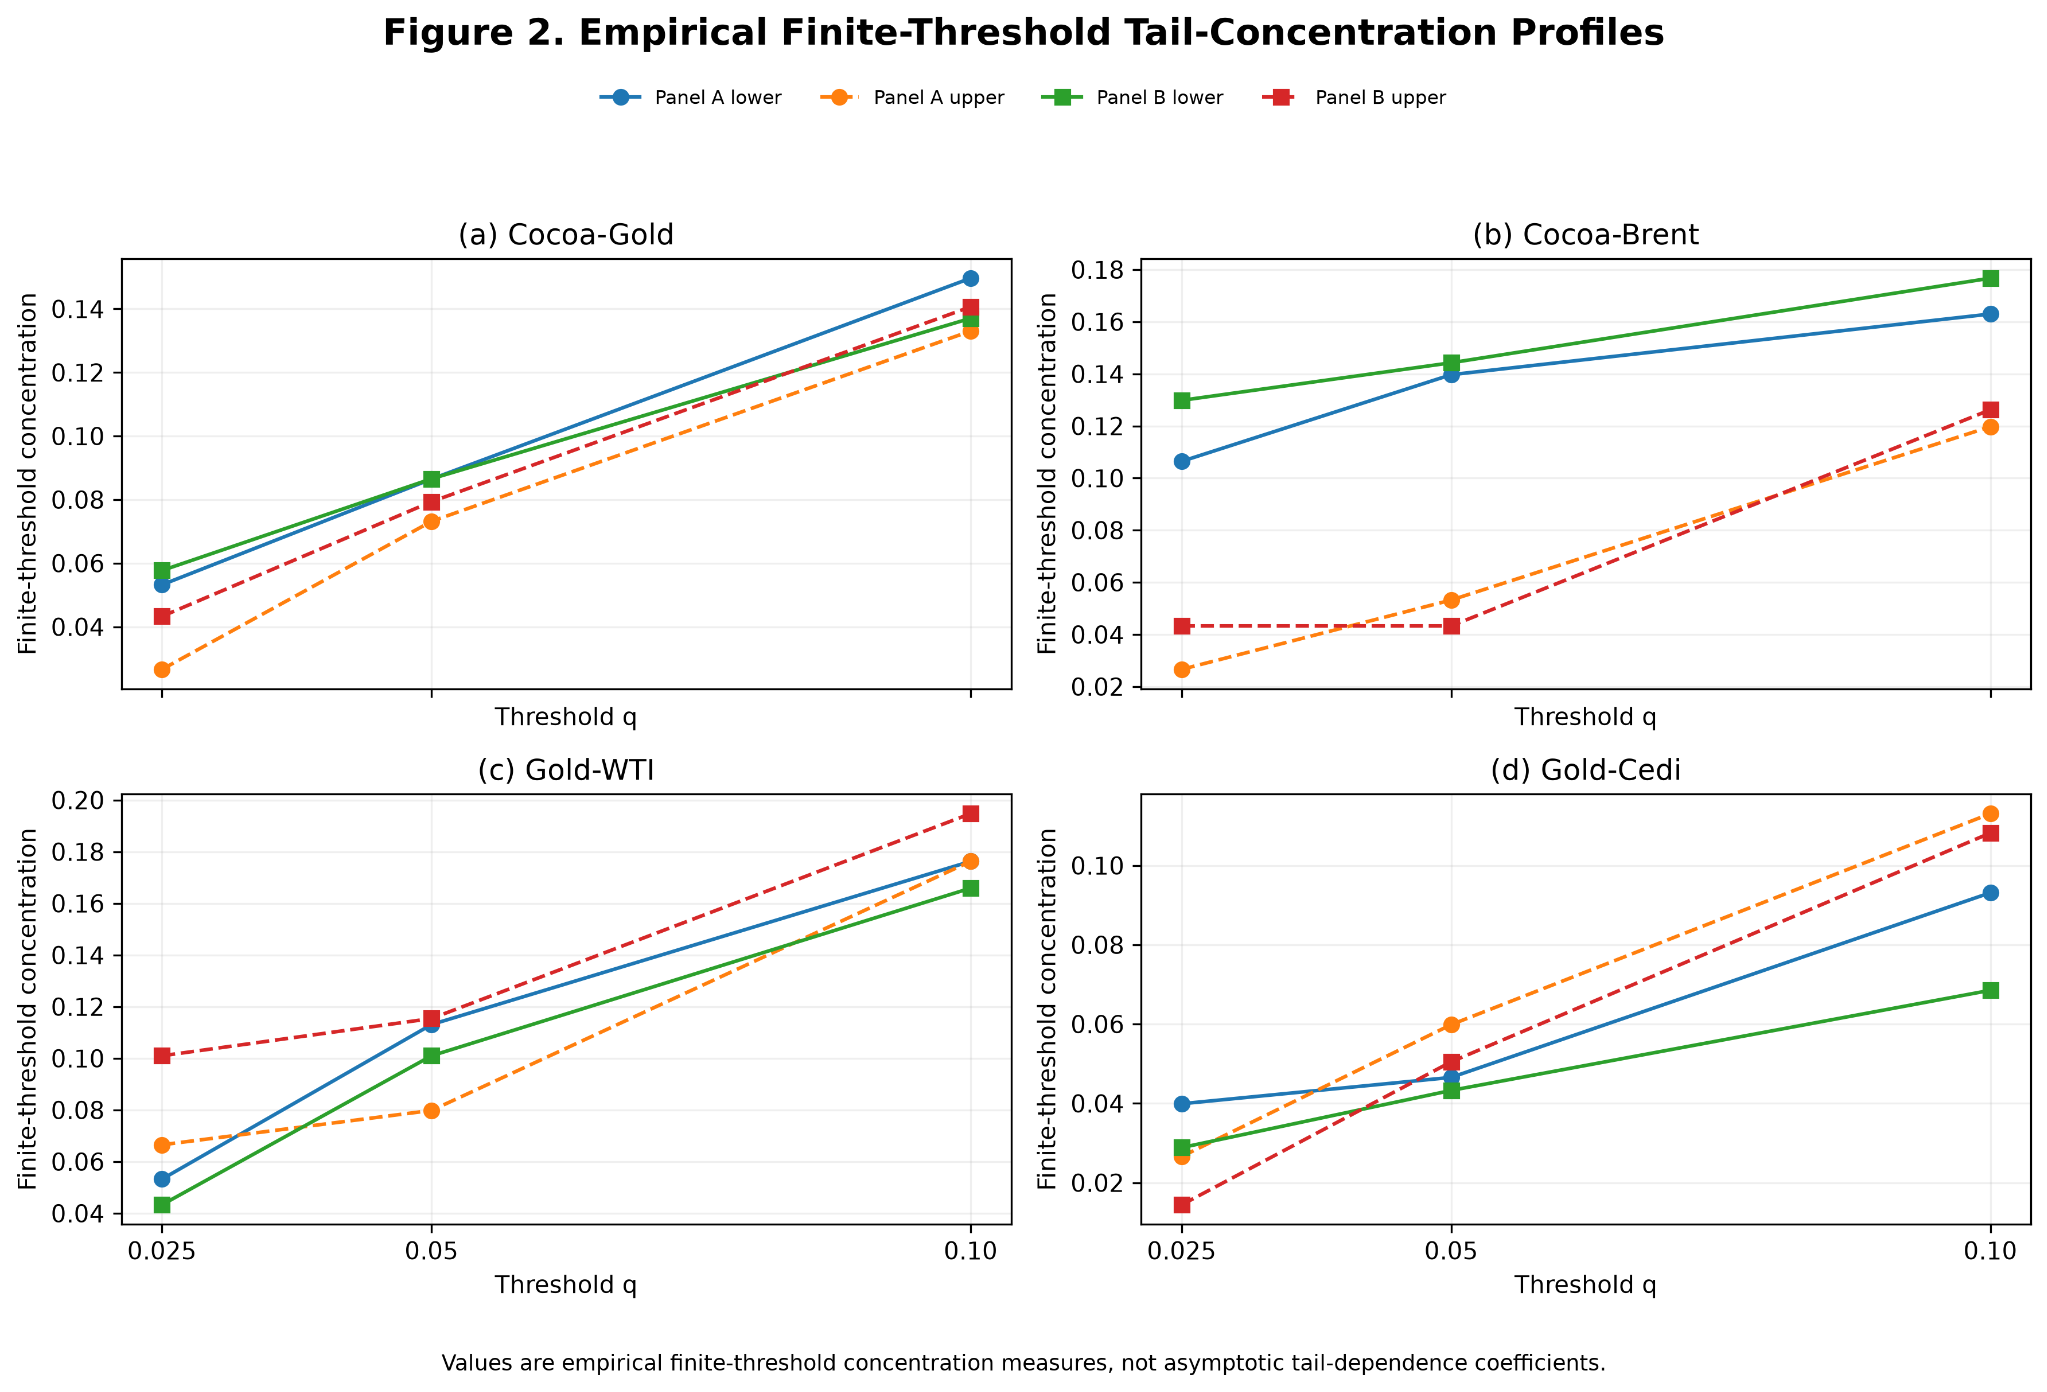
\includegraphics[width=0.98\linewidth]{figures/figure_02_tail_concentration_profiles.png}
\caption{Empirical finite-threshold lower- and upper-tail concentration profiles for selected pairs under the two calendar constructions.}
\label{fig:tail-profiles}
\end{figure}

\subsection{Static copula goodness of fit}

The strongest cross-panel distinction appears in the absolute copula goodness-of-fit results. Table~\ref{tab:gof} reports the number of rejected families, out of the eight tested, for each pair. Gold--Brent, Gold--WTI and Brent--WTI reject all eight families in both panels. These are calendar-robust rejections of the entire tested static family set.

The four commodity--cedi pairs show the opposite classification: none of the eight tested families is rejected for Cocoa--Cedi, Gold--Cedi, Brent--Cedi or WTI--Cedi in either panel. This is also calendar-robust, but it is interpreted cautiously because all four cells depend on the inadequate cedi marginal reference model. Non-rejection does not establish that the families are correct or equally plausible.

The three cocoa-related commodity pairs are calendar-sensitive. Cocoa--Gold, Cocoa--Brent and Cocoa--WTI reject all eight families in Panel A, whereas Panel B rejects only two of eight families for Cocoa--Gold and three of eight for Cocoa--Brent and Cocoa--WTI. Thus the adequacy conclusion for these pairs changes materially with the observation calendar even though the corresponding return series remain closely related across panels.

\begin{table}[htbp]
\centering
\caption{Static copula goodness-of-fit classifications across calendar constructions.}
\label{tab:gof}
\small
\begin{tabularx}{\textwidth}{lccX}
\toprule
\textbf{Pair} & \textbf{Panel A rejected} & \textbf{Panel B rejected} & \textbf{Classification} \\
\midrule
Cocoa--Gold & 8/8 & 2/8 & Calendar-sensitive \\
Cocoa--Brent & 8/8 & 3/8 & Calendar-sensitive \\
Cocoa--WTI & 8/8 & 3/8 & Calendar-sensitive \\
Cocoa--Cedi & 0/8 & 0/8 & Calendar-robust non-rejection \\
Gold--Brent & 8/8 & 8/8 & Calendar-robust rejection \\
Gold--WTI & 8/8 & 8/8 & Calendar-robust rejection \\
Gold--Cedi & 0/8 & 0/8 & Calendar-robust non-rejection \\
Brent--WTI & 8/8 & 8/8 & Calendar-robust rejection \\
Brent--Cedi & 0/8 & 0/8 & Calendar-robust non-rejection \\
WTI--Cedi & 0/8 & 0/8 & Calendar-robust non-rejection \\
\bottomrule
\end{tabularx}
\end{table}

\begin{figure}[htbp]
\centering
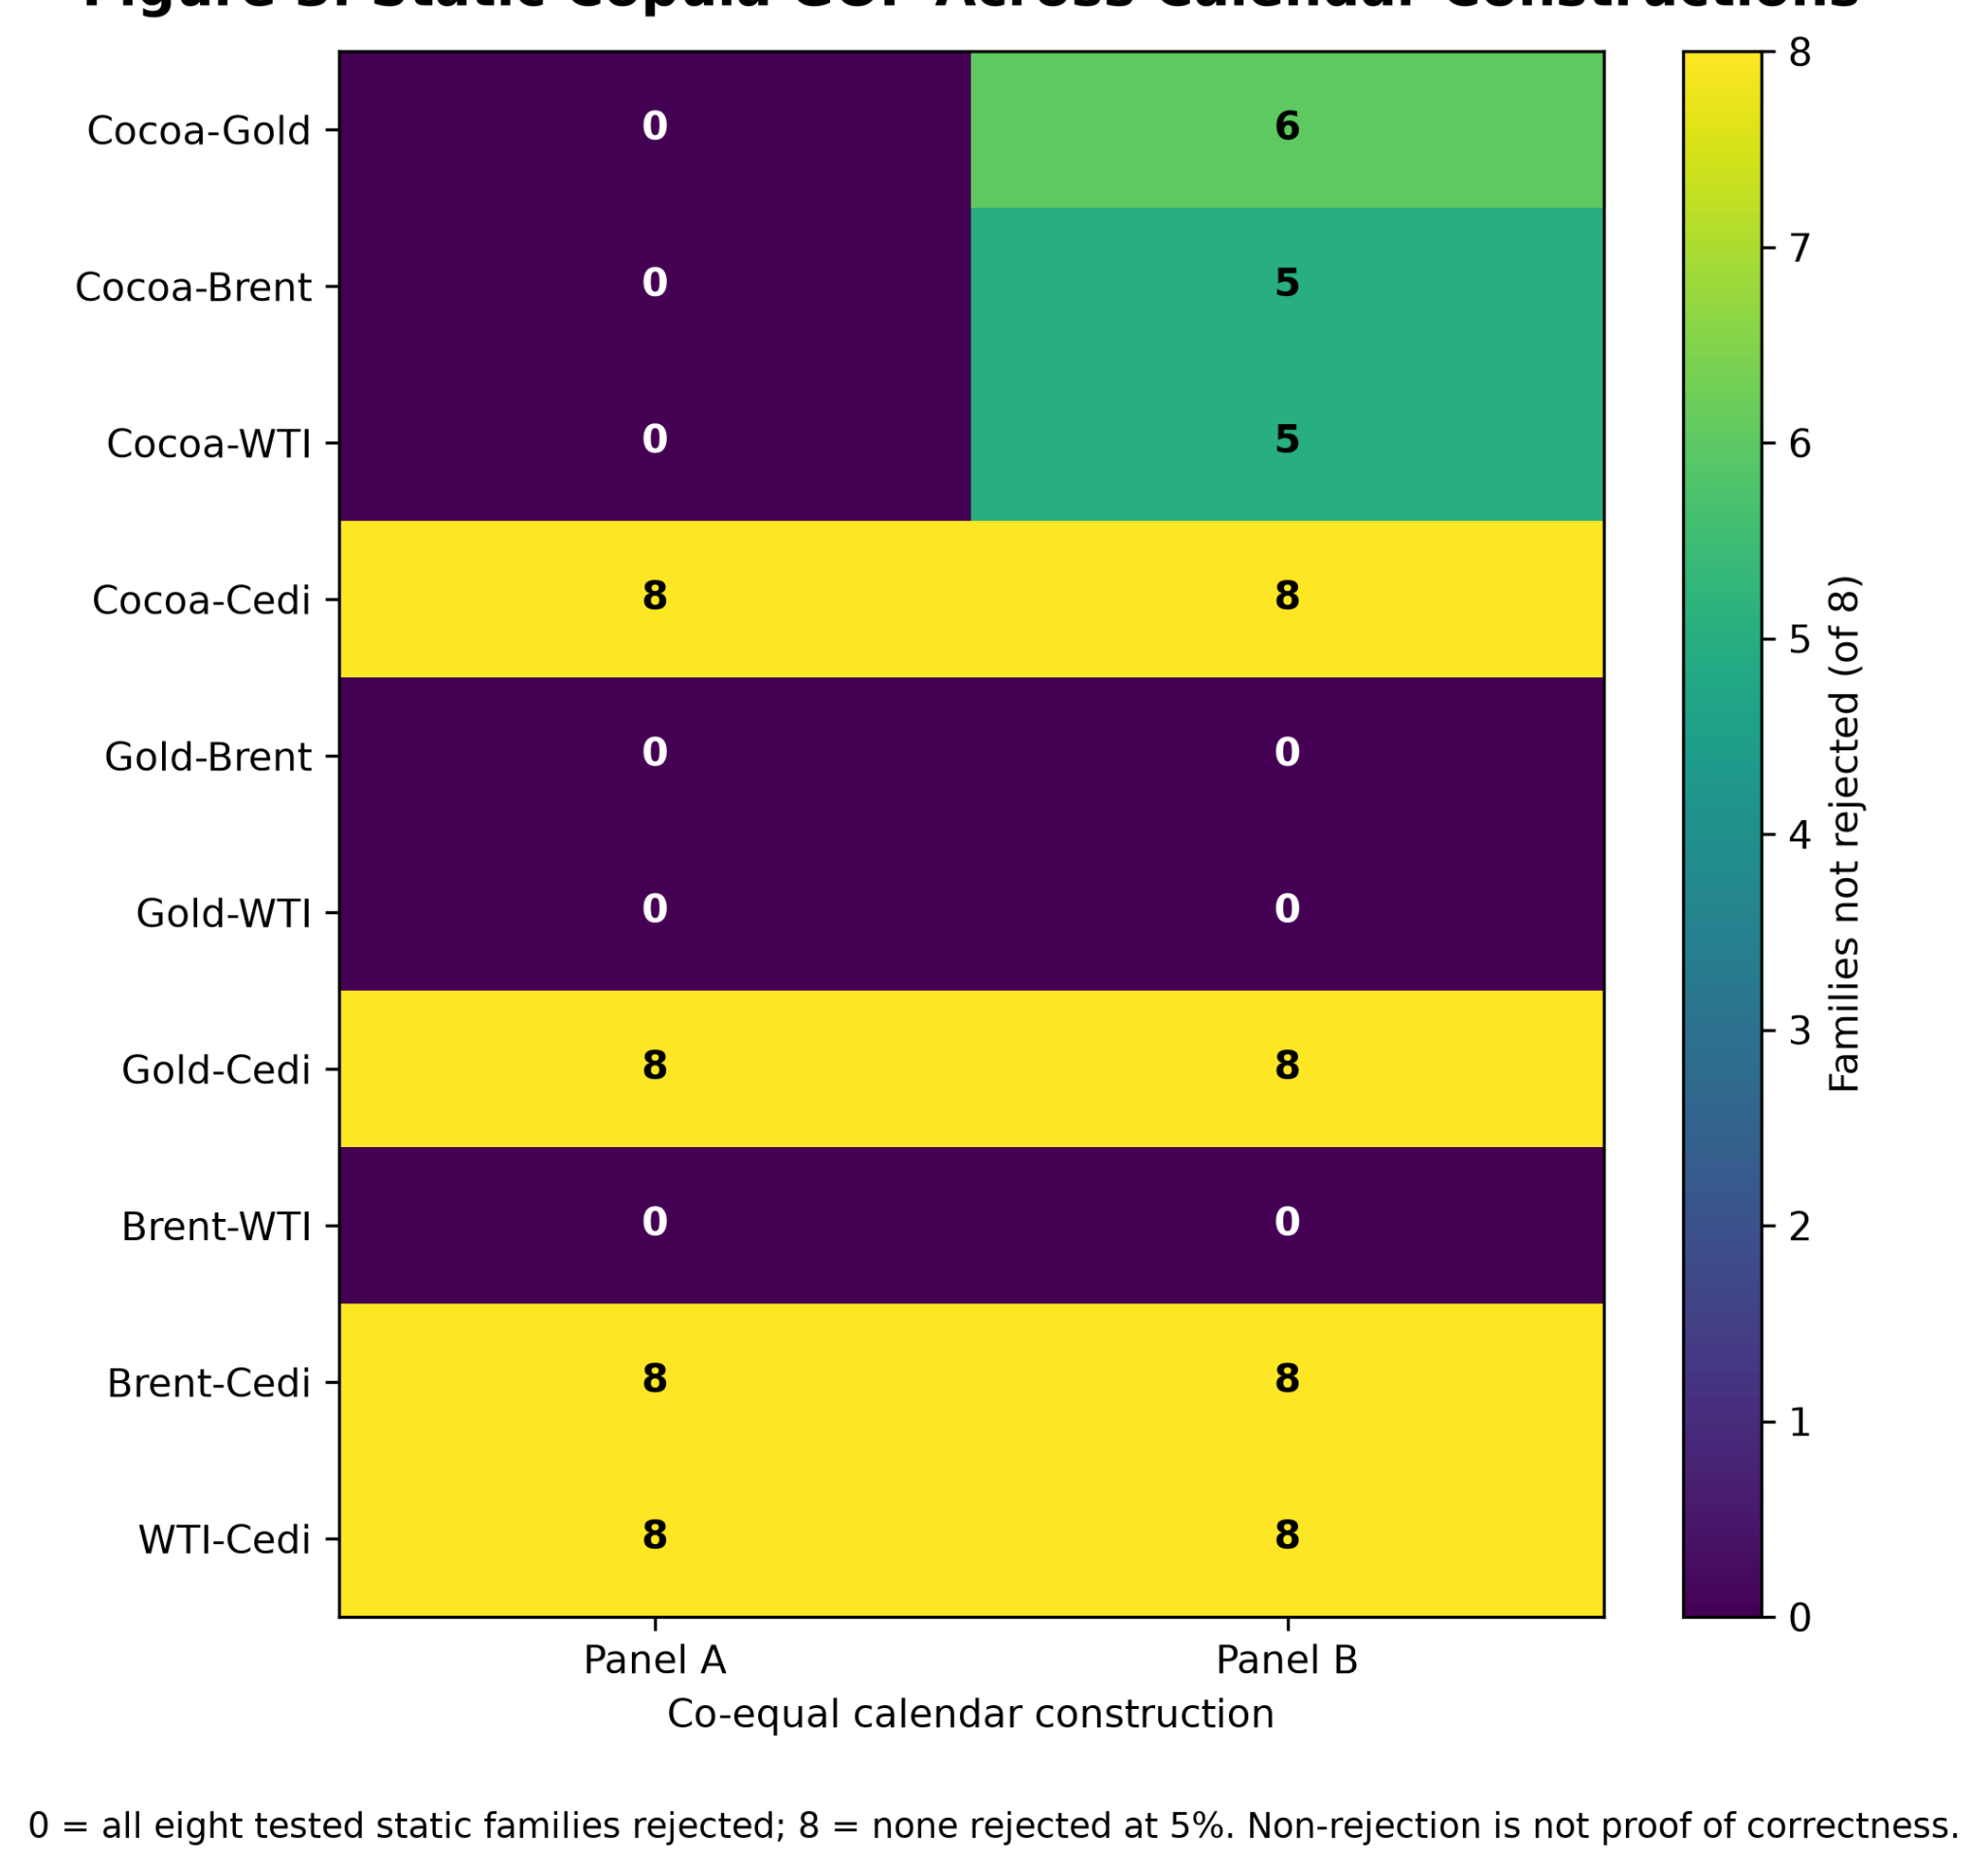
\includegraphics[width=0.96\linewidth]{figures/figure_03_copula_gof_heatmap.png}
\caption{Static copula goodness-of-fit across the two calendar constructions. Each cell reports the number of the eight tested families not rejected at the 5\% level.}
\label{fig:gof-heatmap}
\end{figure}

Figure~\ref{fig:gof-heatmap} displays the same pattern using the number of families not rejected. The contrast between the robust commodity-only rejection cells, the calendar-sensitive cocoa cells and the commodity--cedi non-rejection cells is visible without selecting a single ``best'' copula.

\subsection{Stress--calm inference}

Nominal stress evidence is present in both panels, but none survives multiplicity control. For the Combined stress definition, Panel A contains 6 nominal \(p<0.05\) cells and Panel B contains 5. COVID-19 alone produces 13 nominal findings in Panel A and 11 in Panel B. The 2024 definition produces 6 in Panel A and 7 in Panel B. After either Bonferroni or Benjamini--Hochberg adjustment, the number of discoveries is zero for every panel-by-stress family.

\begin{table}[htbp]
\centering
\caption{Nominal and multiplicity-controlled stress--calm test counts.}
\label{tab:stress}
\small
\begin{tabular}{lcccc}
\toprule
\textbf{Stress definition} & \textbf{A nominal} & \textbf{B nominal} & \textbf{Bonferroni A/B} & \textbf{BH A/B} \\
\midrule
Combined & 6/60 & 5/60 & 0/60; 0/60 & 0/60; 0/60 \\
COVID-19 & 13/60 & 11/60 & 0/60; 0/60 & 0/60; 0/60 \\
2024 & 6/60 & 7/60 & 0/60; 0/60 & 0/60; 0/60 \\
\bottomrule
\end{tabular}
\end{table}

\begin{figure}[htbp]
\centering
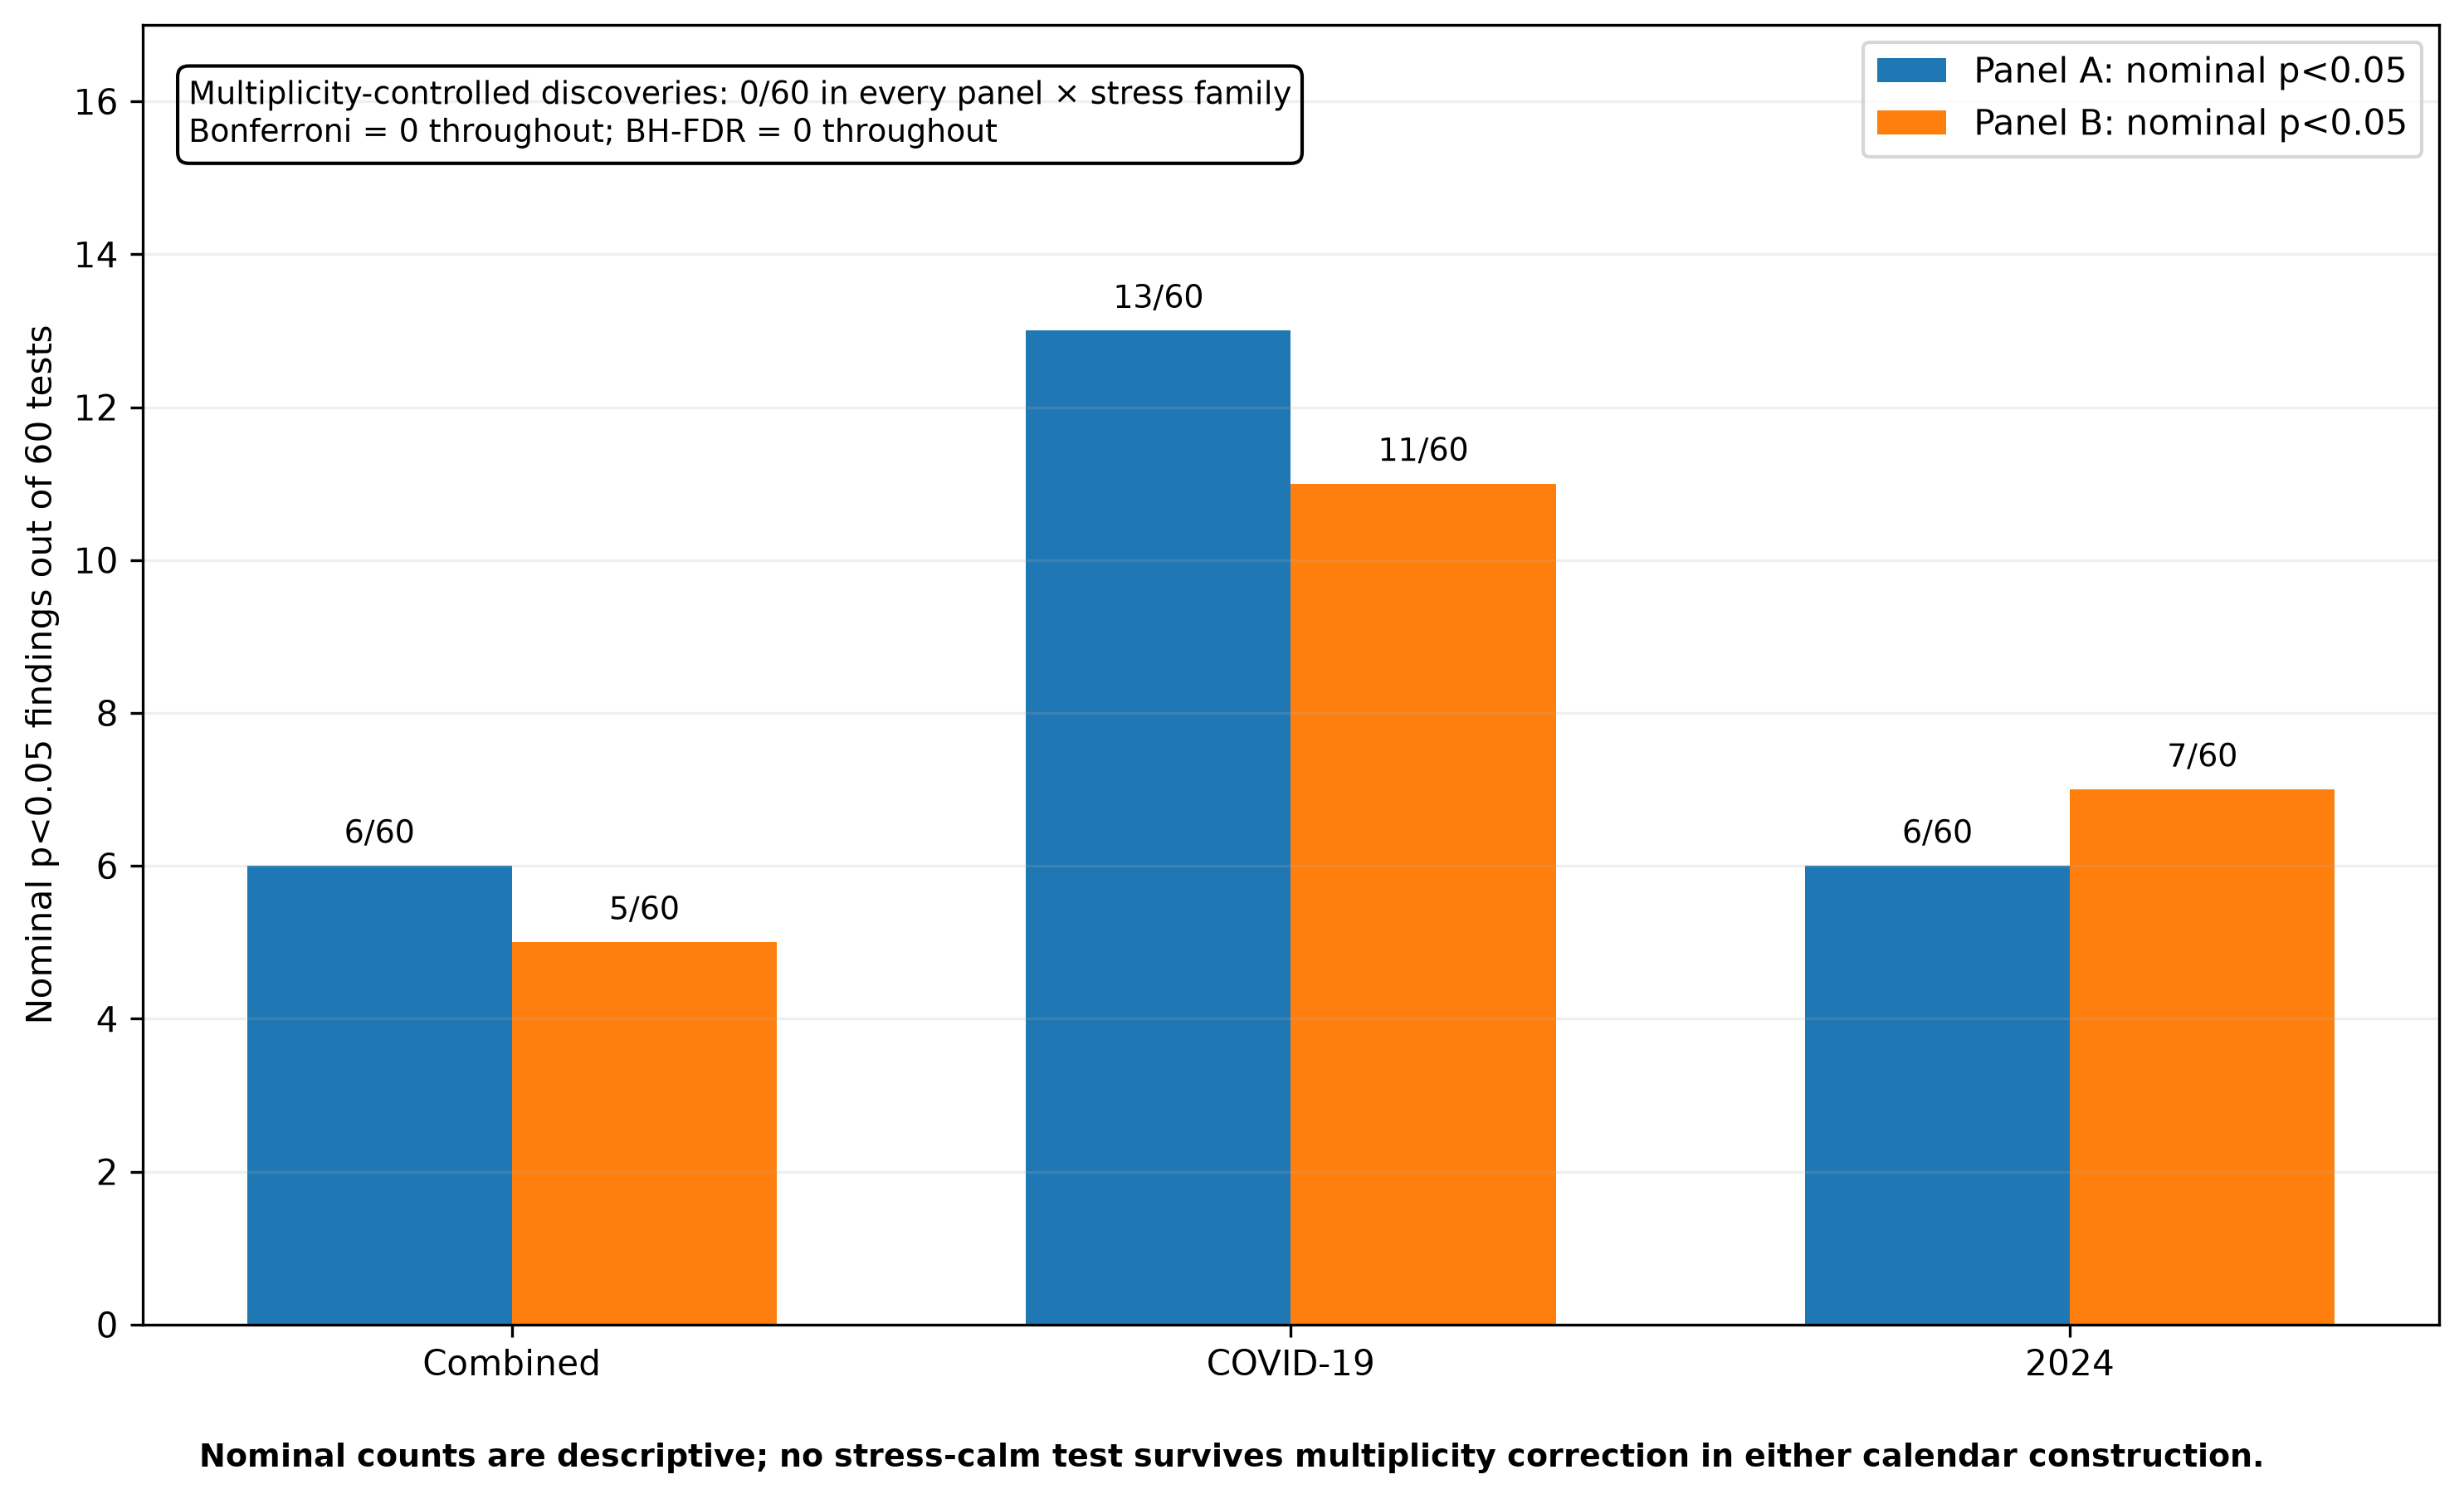
\includegraphics[width=0.92\linewidth]{figures/figure_04_stress_summary.png}
\caption{Nominal versus multiplicity-adjusted stress--calm findings across the two calendar constructions.}
\label{fig:stress-summary}
\end{figure}

The inferential conclusion is therefore calendar-robust: the tested stress-versus-calm differences do not provide corrected evidence strong enough to support an individual tail-concentration change under the prespecified thresholds, windows and bootstrap design. This statement is deliberately narrower than saying that market dependence was unchanged during COVID-19 or 2024.

\subsection{Cedi diagnostics}

The cedi remains the principal marginal-model limitation. The Panel B 90th-percentile POT/GPD fit gives approximately \(\hat\xi=0.693\) and \(\hat\beta=0.329\), with 99\% VaR of about 2.332 and 99\% expected shortfall of about 7.616 in standardized-residual units. Across threshold quantiles from 0.85 to 0.975, the fitted cedi shape parameter remains positive, approximately 0.63--0.79. These values are consistent with a heavy fitted loss tail under the retained reference process, but they are not treated as a model-free structural tail index because the cedi margin fails the PIT adequacy gate.

Supplementary diagnostics reinforce that caution. The Panel A clipping artifact affects only two pseudo-observations after the underlying order is recovered, leaves membership in the \(q=0.025\), \(0.05\) and \(0.10\) tail sets unchanged, and changes the largest observed cedi-pair GOF statistic by only about 0.000262. Alternative cedi treatments also show that nominal daily commodity--cedi patterns are not invariant to modeling and frequency choices. The main cedi limitation is therefore the inability of the tested continuous marginal models to reproduce the zero-heavy daily process adequately, not the numerical clipping step.

\subsection{Cross-panel synthesis}

Three results summarize the empirical evidence. First, Gold--Brent, Gold--WTI and Brent--WTI exhibit calendar-robust rejection of all eight tested static copula families. Second, Cocoa--Gold, Cocoa--Brent and Cocoa--WTI exhibit calendar-sensitive copula adequacy. Third, no stress family produces a multiplicity-adjusted discovery in either panel. Commodity--cedi non-rejection is also stable across calendars, but because the cedi marginal is inadequate in both panels, those results remain conditional diagnostics rather than strong evidence of correct copula specification.
